
\section*{Learning Objectives}

\begin{itemize}
\item What is coding?
\item Getting started with coding at the level of a calculator.
\end{itemize}

\section*{Outcomes} 
\begin{itemize}
\item The Good, The Bad, and the Ugly about Julia
\item What is rounding error
\item Assigning variables
\item Basic arithmetic 
\item Our first dive into an error message
\item A list of built-in functions
\item Rebooting: what to do when all else fails
\item How to learn and keep track of programming skills
\end{itemize}


\newpage

\begin{figure}[htb!]%
\centering
\subfloat[]{%
    \label{fig:LiDARmap}%
	\centering
	\setlength{\fboxsep}{0pt}%
\setlength{\fboxrule}{3pt}%
\fbox{

\includegraphics[width=0.25\columnwidth]{Chap00/IllumiDeskLink.png}}%
}
\hspace{5pt}%
\subfloat[]{%
    \label{fig:Regression}%
	\centering
		\setlength{\fboxsep}{0pt}%
\setlength{\fboxrule}{3pt}%
	\fbox{

\includegraphics[width=0.7\columnwidth]{Chap00/StartMyServer.png}}%
}
\hspace{5pt}%
\subfloat[]{%
    \label{fig:Segway}%
	\centering
			\setlength{\fboxsep}{0pt}%
\setlength{\fboxrule}{3pt}%
	\fbox{
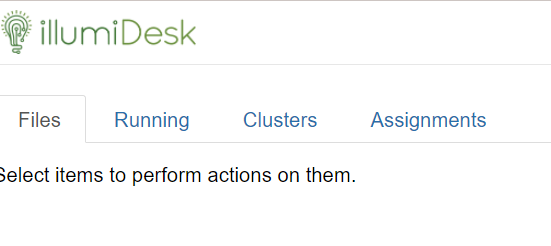
\includegraphics[width=0.35\columnwidth]{Chap00/AssignmentsTab.png}}%
}
\hspace{5pt}%
    \subfloat[]{%
    \label{fig:GradientDescentIntro}%
	\centering
			\setlength{\fboxsep}{0pt}%
\setlength{\fboxrule}{3pt}%
	\fbox{
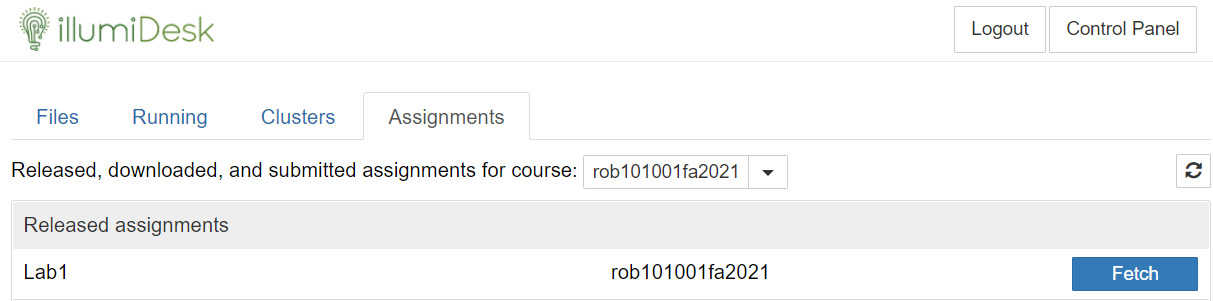
\includegraphics[width=0.6\columnwidth]{Chap00/FetchButton.png}}%
}
\hspace{5pt}%
\subfloat[]{%
    \label{fig:CameraCalibration}%
	\centering
			\setlength{\fboxsep}{0pt}%
\setlength{\fboxrule}{3pt}%
	\fbox{

\includegraphics[width=0.9\columnwidth]{Chap00/DownloadedAssignments.png}}%
}
\hspace{5pt}%
\subfloat[]{%
    \label{fig:ResistorOpAmp}%
	\centering
			\setlength{\fboxsep}{0pt}%
\setlength{\fboxrule}{3pt}%
	\fbox{
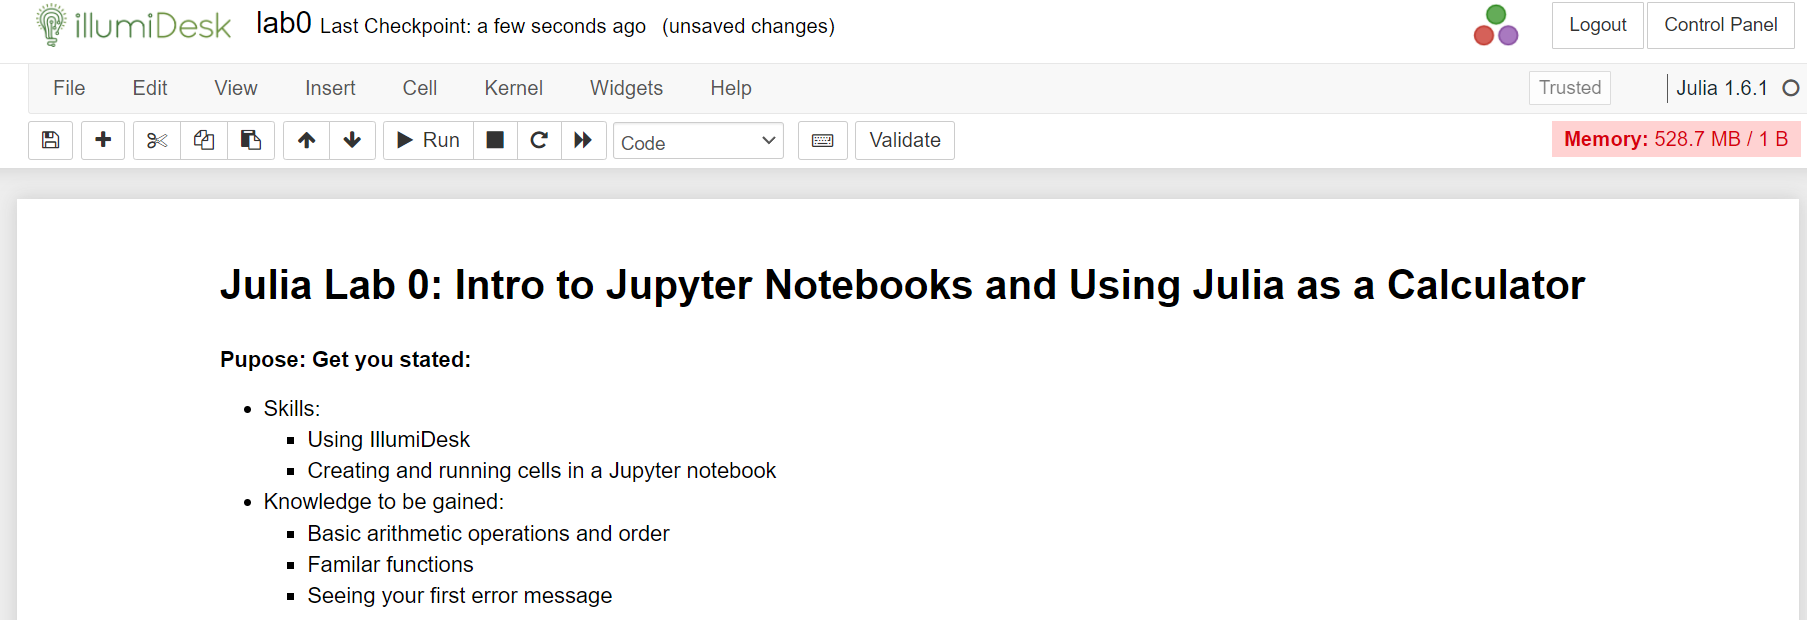
\includegraphics[width=0.8\columnwidth]{Chap00/Lab00Header.png}}%
}
    \caption[]{Sequence of steps for accessing your Julia assignments. (a) You start in Canvas, where you click the IllumiDesk link on the left hand side of the page. (b) Once in IllumiDesk, start your sever! (c) Go to the assignments tab. (d) Fetch the assignment. (e) Click on the name of the assignment. \textcolor{red}{\bf For Labs, you never use the submit button. Labs are not graded.}  \textcolor{blue}{\bf Labs are meant to help you with the Julia HW sets, which are graded.} (f) View of a Jupyter notebook.}
    \label{fig:IllumiDesk}
\end{figure}

\section{Welcome to ROB 101 and the Julia Programming Language!}

ROB 101 assumes no prior experience with Calculus or programming. These notes are meant for the novice programmer. Learning to code is both fun and frustrating at the same time. Our goal with these notes is to increase the amount of time you have fun and reduce the frustration to the minimum necessary for learning to take place. We all had to touch a hot stove once in our lives! \\ %

If you took programming in High School (HS) or you've already taken ENGR 101 at Michigan, then you have a head start, perhaps. I say perhaps, because Julia is similar to MATLAB, and being a pretty good MATLAB programmer, I expected to pick up Julia in a flash. Wrong! There are just enough maddening differences that I was super frustrated for the first month to six weeks. The same will be true of those of you who know C++. To help you out, in the Appendix, you will find helpful hints to speed your transition into Julia. You can find many sites like this one for additional help \url{https://github.com/brenhinkeller/JuliaAdviceForMatlabProgrammers}. When you find even better sites, please let us know.\\

If you did not take programming in High School, these notes are meant for you! You'll find that learning math and programming at the same time is a much richer and more meaningful experience than learning math alone. My colleague Prof Chad Jenkins coined the phrase, ``Programming = Believing'', and I think he is right. Our goal is to turn into code almost every equation we see in lecture. Things we would never ever dream of doing by hand become ``cake'' in Julia. \\

\textbf{Why are we using Julia?} For several reasons:
\begin{itemize}
    \item Robotics is working alongside Historically Black Colleges and Universities (HBCUs) \url{https://en.wikipedia.org/wiki/Historically_black_colleges_and_universities}, and eventually other Minority Serving Institutions (MSIs), to offer Robotics instruction either remotely or in house. To support remote instruction, we wanted a programming language that we could deliver via a browser. While most students at engineering-intensive universities can download MATLAB to a laptop for free, that is not true at most institutions of higher learning. 
    \item Julia is open source and hence free to everyone! Robotics is a huge supporter of the open-source movement. Even as a Michigan student with free access to MATLAB, when you leave Michigan, there is no guarantee that your company will have MATLAB because it is quite expensive (multiple thousands of dollars per user (seat)). Because Julia is free, cost is not a limiting factor for its adoption. 
    \item Julia is blazingly fast. When you run a block of code for the first time, it is compiled. Thereafter, you essentially have the speed associated with C++.
    \item Julia is modern and forward looking. As someone who was taught FORTRAN back in the day, it feels good to be sharing with you a language that is likely to stand a significant test of time. 
\end{itemize}

\textbf{Why should we have chosen anything but Julia for ROB 101?} The error messages in Julia are horrible. These will be fixed in Julia 2.0. The most current release is Julia 1.6 and thus we'll have to teach you how to suffer through the error messages and find your mistakes. A second reason would be that Julia is \emph{strongly typed}, which is the proverbial ``blessing'' and a ``curse''. \\


For the super nerds, you must know about the official website for the Julia programming language \url{https://julialang.org/}. It's promotion of Julia is designed for professional programmers. There is a blog that is kind of fun \url{https://julialang.org/blog/2022/02/10years/} where a group of Julia founders and pioneers look back on the language. \\

All of the Julia work for ROB 101 can be completed in the cloud via a browser. \textbf{You do not need to install Julia on your personal computer! You can complete the assignments with as little as an iPad and a mouse.} Nevertheless, some of you may want to have your own Julia installation; see  Appendix~\ref{App:MyOwnJulia} for how to do that. If you pursue your own installation, \textbf{we cannot provide IT support. We do not have the person-power to do it.} \textcolor{red}{\bf Moreover, you cannot submit HW or Project assignments from your personal Julia installation.} While you can transfer files from IllumiDesk to a  personal installation, do the work there, and then copy your work \textbf{cell by cell} to the IllumiDesk environment, you may find that very tedious. You might, however, create your own installation so that you can work on Julia when you are ``off the grid'', for example, or because ``you like the feel of being in control of your computing environment''. 


\section{Vocabulary}

\begin{itemize}
    \item \textbf{Programming} is the act of writing instructions for a computer to follow. \textbf{Coding} is similar to programming...if there is a difference, it would be that you do not ``code'' a computer, you ``program'' it, while the action of writing or composing computer instructions can be called either ``coding'' or ``programming''. 
    \item \textbf{Syntax} is the set of formal rules that govern a language, whether a human language such as Spanish or English, or a computer language, such as Julia or C++. Syntax prescribes the allowed symbols in a language, how they can be combined/ordered, and the role of punctuation. Where a pair of square brackets $[~~~ ]$ is used in Julia to ``index'' or ``slice'' an array of numbers, in MATLAB, one uses instead parentheses $( ~~~ )$. These differences can be maddening, just like ``false friends'' between English and French, such as the word ``special'' having a positive connotation in English and ``speciale'' having a negative connotation in French. How can that be? Or French inserting a space before a question mark at the end of a sentence, while in English, we do not. The challenge with learning a computer language is that it is \textbf{unforgiving of syntax errors}. If you are lucky, it ``throws an error flag'' and identifies the line on which the error occurred. If you are unlucky, what you entered was still legal syntax and the computer does something you never intended, without you suspecting that your instruction actually meant something else. 
    \item A list of \textbf{punctuation symbols} in Julia \url{https://docs.julialang.org/en/v1/base/punctuation/}. We will only encounter a few of them in ROB 101.
    \item \textbf{Debugging} computer code is the process of finding and fixing errors in the code. It could be that the code does not run because the errors were ``fatal'' or the code runs but produces flawed output. You can read more here about the etymology of the term debugging \url{https://en.wikipedia.org/wiki/Debugging}. 
    \item \textbf{Variables} store information that can be referenced or changed in a program; see \url{https://en.wikipedia.org/wiki/Variable_(computer_science)}.
    \item A variable's \textbf{Type} determines the values it can hold and the operations that can be performed on the variable. If a variable's type is \texttt{char} then it can hold characters, such as letters of the alphabet, or common symbols such as $@$ or $\&$. If its type is \texttt{char} and you try to assign a real number to it, you will generate an error. In the computer, a variable's type is used to economize on storage space, because in general it takes more zeros and ones (\textbf{bits}) to specify a real number than it does a letter of the alphabet. Hence allocating a ton of space in memory and then putting the letter D in it is wasteful. Types are also used to indicate what operations can be performed on a variable. For example, letters in the alphabet (variables of \texttt{char} type) can be concatenated to form \texttt{strings}, whereas it does not make so much sense to concatenate $3.14159$ with $1.41421$, because what would you do with an object that had two decimal points? Similarly, it makes sense to add two real numbers (type \texttt{Real}), but not so much the addition of two letters A and M. By assigning \texttt{Types} to all variables, Julia helps you to avoid ``stupid mistakes''. We'll also see that Julia can sometimes be so strict with its imposition of \texttt{Types} that it's maddening. More on this later.
    \item \textbf{Jupyter Notebook} (spelling is correct) ``is an open-source web application that allows data scientists to create and share documents that integrate live code, equations, computational output, visualizations, and other multimedia resources, along with explanatory text in a single document\footnote{\url{https://odsc.medium.com/why-you-should-be-using-jupyter-notebooks-ea2e568c59f2}}.'' Jupyter is sort of a contraction built from the programming languages Julia, Python, and R.  Jupyter Notebooks consist of a sequence of cells, where each cell can hold code, text, plots, typeset equations, images, etc.
    \item \textbf{IllumiDesk} is the company supporting our web access to Julia and Jupyter notebooks; you can learn more at \url{https://www.illumidesk.com/}. 
     \item A more extensive \textbf{glossary of coding terminology} is available here \url{https://code.org/curriculum/docs/k-5/glossary}. 
\end{itemize}

\section{Accessing Julia HWs and Labs via IllumiDesk}
\label{sec:IllumiDesk}

IllumiDesk is accessed via the ROB 101 Canvas page; hence you need to be a member of the course's Canvas site to reach it. Once you login to Canvas, you want to 
\begin{itemize}
    \item Click on the IllumiDesk link in the left hand panel
    \item Hit the big blue \textcolor{blue}{\bf Start My Server} button.
    \item Click on the assignment tab
    \item Click on the \textcolor{blue}{\bf Fetch} button  for the appropriate assignment.
    \item Look below to the Downloaded Assignments area and click on the appropriate link. You may need to scroll down the page a bit to see the Downloaded Assignments area.
    \item You should now be in a Jupyter notebook; see Fig.~\ref{fig:IllumiDesk}.
\end{itemize}


\section{Learning and Keeping Track of Programming Skills}
\label{sec:GoogleDoc4Commands}

%\vspace*{.2cm}

While we have summarized the most frequently used commands in Appendix~\ref{App:JuliaCommands}, you will learn more quickly if you create your own record of frequently used commands and encountered problems. It is suggested that you make a copy of the following Google Doc \url{https://docs.google.com/document/d/1NnB0dFUKbLAOJ8CIB9YpXj71XhAPFwmTAYOFDDDHR_w/edit?usp=sharing} and add commands to it as you learn them in the course. You must make your own personal copy before you can edit the file. Once you copy the file, you can rename it and add content.\\

Can a group of you share a Google Doc filled with Julia tips and tricks? Sure. It's OK, but you'll probably learn more if you make your own ``cheat sheet''.


\vspace*{.2cm}
\setlength{\fboxrule}{3pt}%
	\centerline{ \fbox{ 
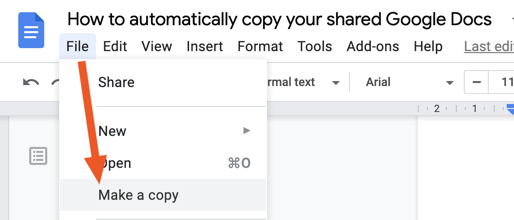
\includegraphics[width=0.5\columnwidth]{Chap00/WildRobotTeacherGuide.png}}%
}

\section{LAB 0: Julia as a Calculator}

This lab gets you started with Julia. You should follow the steps in Chapter~\ref{sec:IllumiDesk} and open the lab0 Julia notebook, or in your own installation of Julia, open a Julia notebook and try the various basic commands introduced here.\\

\setlength{\fboxrule}{3pt}%
	\centerline{ \fbox{ 
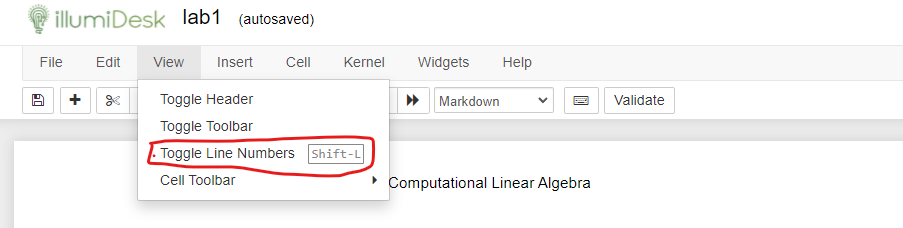
\includegraphics[width=0.9\columnwidth]{Chap00/LineNumbers.png}}%
}



\begin{rem} \textbf{(Enable Line numbering)} \texttt{View > Toggle Line Numbers}. In labs and on homework assignments, you will come across instructions which tell you to alter certain lines of your code. You will also need to debug your code based on the errors reported by Julia, which will tell you the line number at which your program failed. 
\end{rem}

If you are in a Jupyter notebook and want to \textbf{create a new cell}, hit the plus sign  \Plus ~in the top banner. The cell will open below the cell in which you last clicked with your cursor (play around with it). This works for HW, LABs, and empty Jupyter notebooks. If you want to try something out, such as rewriting a piece of code without erasing your current code, just open a new cell below the current one, copy and paste in whatever you wish and go to work. To \textbf{remove a cell}, click on it with your cursor, and then click on the scissor symbol \ScissorHollowRight, which is right next to the plus sign \Plus. To \textbf{run a cell}, you hit the run button $\blacktriangleright$~\texttt{Run} button on the top banner. On a PC, you can hold \texttt{Shift Enter}. It is worth getting to know the family of buttons on the top banner. Experiment a little! Google a little.\\

\setlength{\fboxrule}{3pt}%
	\centerline{ \fbox{ 
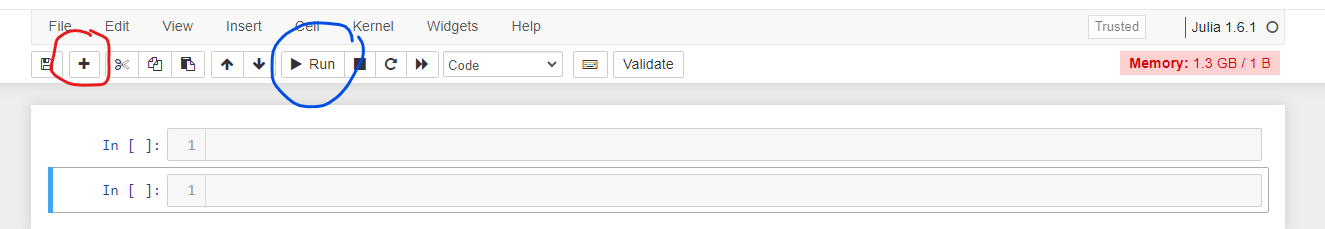
\includegraphics[width=0.9\columnwidth]{Chap00/NewCell.png}}%
}

\subsection{Rounding Error}

\begin{lstlisting}[language=Julia,style=mystyle]
#in a code cell, julia will compute and return operations you do inside it
(1 + 2 + 3 + 4 + 5 + 6)/2
#here is some basic addition followed by division
\end{lstlisting}
\textbf{Output} 
\begin{verbatim}
10.5
\end{verbatim}

Computers do arithmetic with a \textbf{finite number} of zeros and ones.  That's easy to accept. Some of the consequences of doing arithmetic with zeros and ones may be hard to accept when you first start programming. Let's take a look, because \textbf{you probably never noticed what is generally called ``rounding error'' when you used a calculator}. 

\begin{lstlisting}[language=Julia,style=mystyle]
# in a code cell, julia will compute and return operations you do inside it
4+7.62
# basic addition
\end{lstlisting}
\textbf{Output} 
\begin{verbatim}
11.620000000000001
\end{verbatim}
Wait a minute, we're pretty good at arithmetic, ``Julia\footnote{The error has nothing to do with the Julia programming language and everything to do with the binary numbers used in a digital computer.}'' got the wrong answer! It's off by $0.000000000000001 =$ 1e-15 or $1 \times 10^{-15}$. In fact, the actual error is 
\begin{lstlisting}[language=Julia,style=mystyle]
# rounding error
(4+7.62) - 11.62
\end{lstlisting}
\textbf{Output} 
\begin{verbatim}
1.7763568394002505e-15
\end{verbatim}
\textbf{You don't need to understand the source of the error to be successful in ROB 101, but you do need to accept that it occurs.} \\

\textbf{(Optional read:)} \emph{In case you are interested, the \textbf{rounding error} comes from the fact that digital computers do calculations in base 2 using a finite number of zeros and ones.} 
\begin{itemize}
    \item By way of background, you are comfortable with the fraction $\frac{1}{3}$ having the infinite decimal expansion 0.3333333\ldots This means that 
    $$\frac{1}{3} = \sum_{k=1}^\infty\frac{3}{10^k} = \frac{3}{10} + \frac{3}{100} + \frac{3}{1000} +  \frac{3}{10000} +  \frac{3}{100000} +\cdots,$$
    where the $\cdots$ means it goes on forever! Hence, it is not possible to represent the number $\frac{1}{3}$ in decimal notation using a finite number of digits between zero and nine. 
    \item In base 3, however, the decimal fraction $\frac{1}{3}$ has the finite expansion $0.1$, while  $\frac{1}{3} + \frac{2}{3^2} = \frac{5}{9} = 0.555555$ in base 10 has the base 3 expansion 0.12. Finally, $\frac{1}{3} + \frac{2}{3^2} + \frac{1}{3^3}= \frac{16}{27} = 0.592592592$ in base 10, but has the base 3 expansion 0.121.
    \item If you have forgotten or never mastered representing numbers in different bases, then don't worry about it. You can simply accept that a number having a finite (exact) expansion in base 10 does not mean it has a finite (exact) expansion in base 2, the number system used in digital computers.
    \item The number 7.62 requires three digits to express in base 10 (decimal numbers), but it takes an \emph{infinite number of digits} in base 2 (binary numbers). Julia is using something like 111.10011110101110000101 as the binary approximation of 7.62, which is roughly 7.61999988555908203125 in decimal, and is ``very close'' to 7.62, but not equal to it. Indeed, 
\begin{align*}
    \overbrace{111}^{7}.\overbrace{10 01111 01011 10000 101}^{\approx 0.62} =& \overbrace{1 \times 2^2 + 1 \times 2^1 + 1 \times 2^0}^{4 + 2 + 1 = 7} +  \overbrace{ 1 \times 2^{-1} + 0 \times 2^{-2}}^{\text{fraction starts here}} +\\
    &  0 \times 2^{-3} + 1 \times 2^{-4} + 1 \times 2^{-5} + 1 \times 2^{-6} + 1 \times 2^{-7} + \\
     &  0 \times 2^{-8} + 1 \times 2^{-9} + 0 \times 2^{-10} + 1 \times 2^{-11} + 1 \times 2^{-12} + \\
     &  1 \times 2^{-13} + 0 \times 2^{-14} + 0 \times 2^{-15} +0 \times 2^{-16} +0 \times 2^{-17} + \\
     &  1 \times 2^{-18} + 0 \times 2^{-19} + 1 \times 2^{-20} \\
     \approx& 7.619 999 885 559 082 031 25 \\
     =& 7 \times 10^{0} + 6 \times 10^{-1} + 1 \times 10^{-2} + 9 \times 10^{-3} +  9 \times 10^{-4} +  9 \times 10^{-5} + \\
     & \vdots \\
    & 2 \times 10^{-15}+ 0 \times 10^{-16}+  3 \times 10^{-17} +  1 \times 10^{-18}  +  2 \times 10^{-19} +  5 \times 10^{-20}, 
\end{align*}
where the symbol $\approx$ means ``approximately equal to''. This explains the error, in case you care. Understanding ``rounding error'' is not important for ROB 101, but eventually, it becomes important for all students of STEM.
\item If a number has a finite representation in either base 2 or base 5, then it will have a finite representation in base 10, simply because 2 and 5 are factors of 10. For example, 
$$\frac{1}{2^k} = \frac{5^k}{2^k 5 ^k} = \frac{5^k}{10 ^k}.$$
If you stare at this for awhile, you will convince yourself that if in binary, a number has $k$ digits after the ``decimal point'' (binary point?), then in decimal, it will have at most $k$ digits after the decimal point. 
\item Because 3 is not a factor of 10, there is no ``reciprocity'' on finite expansions, as we saw with the fraction $1/3$.    
    \end{itemize}


\begin{notation} In case you are curious, the general name for the point ``\textbf{\large .}'' that separates an integer part of a number from the fractional part is \textbf{radix point} \url{https://en.wikipedia.org/wiki/Decimal_separator}. Not everyone uses points to indicate the separator. The French use a comma to separate the integer part of a number from the fractional part and a period to separate powers of ten. And they are not alone in this practice! Your author did a post-doc in Paris back in the 80's, and had a checking account, of course. Getting the commas and periods correct was slightly important when I wrote a check.
\end{notation}


\subsection{Assignment Operator is Denoted with an Equals Sign}

In mathematics, when we write $x+y+2=3$, we mean the value of the sum of $x$, $y$, and $2$ equals the number $3$. We can ``rearrange'' the equation and write $x + y = 1$ or $x = 1 - y$ without changing what the equation means. \\

In programming, it is very important to understand that the symbol $=$ means \textbf{assignment}. For example, $x=(1 + 2 + 3 + 4 + 5 + 6)/2$ \textbf{assigns} the value 10.5 to the variable $x$. You can now use $x$ in calculations that follow it. It will hold the value 10.5 until you assign something else to it.

\begin{lstlisting}[language=Julia,style=mystyle]
# assigning a value to x
x=(1 + 2 + 3 + 4 + 5 + 6)/2
\end{lstlisting}
\textbf{Output} 
\begin{verbatim}
10.5
\end{verbatim}

\begin{lstlisting}[language=Julia,style=mystyle]
# because we have already assigned x, we can use it in further calculations
y = 3*x
\end{lstlisting}
\textbf{Output} 
\begin{verbatim}
31.5
\end{verbatim}


\begin{lstlisting}[language=Julia,style=mystyle]
# We can update x, using its past value
x = 3*x
\end{lstlisting}
\textbf{Output} 
\begin{verbatim}
31.5
\end{verbatim}

\textbf{The assignment operator does not work like an equals sign.}
\begin{lstlisting}[language=Julia,style=mystyle]
x=x-0.5
\end{lstlisting}
\textbf{Output} 
\begin{verbatim}
31.0
\end{verbatim}
In ``regular'' arithmetic, we could subtract $x$ from both sides of the equation $x=x-0.5$ and arrive at the nonsensical equation, $0=-0.5$. In the computer, you need to think of the left hand side of $x=x-0.5$ as the new value that $x$ will hold. When $x$ appears on the right hand side as well, the computer will use the current value of $x$, which in our case, was $31.5$, perform whatever operations you have specified, and store the new value in $x$. \textbf{In a programming language, $=$ is an assignment operation and not an equals sign.}\\

\begin{rem} \textbf{(Hindsight is 20/20, or the Equals Sign Blues)}
When that first computer programming language was written, there was probably no $\leftarrow$ on the keyboard and hence the notation 
$$ x \leftarrow x+3$$
was not adopted. The left arrow $\leftarrow$ would make a perfectly good assignment operator. In fact, it has been adopted when writing pseudo code \url{https://en.wikibooks.org/wiki/GCSE_Computer_Science/Pseudocode}, which is an informal language, between a human language and a computer language, used for giving the key steps of an algorithm without committing to any particular coding paradigm.
\end{rem}


\subsection{Arithmetic Operations and PEMDAS}

PEMDAS stands for \textbf{P}arentheses, \textbf{E}xponentials, \textbf{M}ultiplication \& \textbf{D}ivision (left to right), \textbf{A}ddition and \textbf{S}ubtraction, the order in which Julia performs operations. While it is fine to memorize this, it is usually better to employ more parentheses than is necessary to make your code easily readable.
\begin{itemize}
    \item Parentheses
\item Exponentials (right to left)
\item Multiplication and Division (left to right)
\item Addition and Subtraction (left to right)
\end{itemize}

\begin{lstlisting}[language=Julia,style=mystyle]
# The symbol ^ means ``raise to the power''
10^(2 + 1)
\end{lstlisting}
\textbf{Output} 
\begin{verbatim}
1000
\end{verbatim}

\begin{lstlisting}[language=Julia,style=mystyle]
# whereas, without parentheses
10^2 + 1
\end{lstlisting}
\textbf{Output} 
\begin{verbatim}
101
\end{verbatim}


\begin{lstlisting}[language=Julia,style=mystyle]
# you can take the power of variables
x = 10 # just to be sure, we set x to a value
x = x^(x^0.5)
\end{lstlisting}
\textbf{Output} 
\begin{verbatim}
1453.0403018990432
\end{verbatim}


% \begin{lstlisting}[language=Julia,style=mystyle]

% \end{lstlisting}
% \textbf{Output} 
% \begin{verbatim}

% \end{verbatim}

\begin{exercise}
Place one (1) set of parentheses in the expression below to make w equal to 30
\begin{lstlisting}[language=Julia,style=mystyle]
#place your parentheses here
w = 2 + 1 + 2 + 7 * 3 
\end{lstlisting}
\end{exercise}

\textbf{Solution:}

\begin{lstlisting}[language=Julia,style=mystyle]
w = 2 + 1 + (2+7)*3 
\end{lstlisting}
\textbf{Output} 
\begin{verbatim}
30.0
\end{verbatim}

\begin{rem} With no parentheses, the result of $w = 2 + 1 + 2 + 7 * 3 $ is $w=26$ because, Julia first does $7 *3=21$ and then performs the addition left to right,  $2 + 1 + 2  + 21 = 26.$

\end{rem}

\begin{exercise}
Place two (2) sets of parentheses in the expression below to make z equal to 7
\begin{lstlisting}[language=Julia,style=mystyle]
#place your parentheses here
z = 2 + 1 + 2 + 7 * 3 + 2 / 10 + 2
\end{lstlisting}
\end{exercise}

\textbf{Solution:}

\begin{lstlisting}[language=Julia,style=mystyle]
z=2 + (1 + (2+7)*3 + 2)/10 + 2
\end{lstlisting}
\textbf{Output} 
\begin{verbatim}
7.0
\end{verbatim}

\begin{rem}
Adding parentheses to someone else's equation is no fun! Your instructor hates those kinds of problems. The take-home point is that parentheses allow you to control the order of computations. If you did not find the solution to the problem on your own, no worries. 
\end{rem}

\begin{rem} With no parentheses, the result of $z = 2 + 1 + 2 + 7 * 3 + 2 / 10 + 2$ is $z=28.2$ because, Julia first does $7 *3=21$ and 2/10 = 0.2, before then performing the addition left to right,  $2 + 1 + 2  + 21 + 0.2 + 2= 28.2.$
\end{rem}



\subsection{Reading an Error Message}

You are going to make lots of errors. Let's make an error on purpose to see what happens. It is assumed that you have not yet defined a value to the variable $r$. If you have used $r$, replace it in the following with something else, like $rr$.

\begin{lstlisting}[language=Julia,style=mystyle]
# A deliberate error
r = r+2
\end{lstlisting}
\textbf{Output} 
\begin{verbatim}
UndefVarError: r not defined

Stacktrace:
 [1] top-level scope
 @ In[15]:2
 [2] eval
   @ ./boot.jl:360 [inlined]
 [3] include_string(mapexpr::typeof(REPL.softscope), mod::Module, code::String,
 filename::String)
   @ Base ./loading.jl:1094
\end{verbatim}

Julia reported that $r$ is an \textbf{undefined variable} via the statement \texttt{UndefVarError: r not defined}. That's cool, you now know the name of the problematic variable and the nature of the problem. You were next told in which cell of your Jupyter notebook the error occurred, here it was input cell 15, and the line number of the cell in which the error occurred, here it was line 2. You can see all of this that from the line \texttt{@ In[15]:2}. The other parts of the error message are helpful for a Julia professional, but not so much for us. Once again, the key parts of the error message are \newline
\textcolor{blue}{\bf Stacktrace:}\newline
 \textbf{[1] top-level scope} \newline
\textcolor{red}{\bf @ In[15]:2 ~~$\leftarrow$ gave the Jupyter Cell number and the line number in the cell where the error occurred.} When you compose more complicated notebooks, the Cell number may be further up in your jupyter notebook, possibly where you define a new function. Julia's error messages can be called lot's of things, cryptic and arcane would be two of the nicer ones. Oh well! \textbf{Always look for the line that has \texttt{In[ some cell number ]: some line number } to get started on locating your error.} And of course, have line numbering turned on.


\section{Standard Bulit-in Functions}

As you can imagine, Julia has many built-in functions, more than a standard calculator will have. Here are a few,
\begin{itemize}
\item abs() \#absolute value
\item sin(), cos(), tan(), asin(), acos(), atan()  \#many more trigonometric functions
\item sqrt() \#square root
\item exp()  \#natural exponential $e^x$
\item log() \#natural logarithm
\item round() \#rounds to nearest integer
\item ceil() \#rounds up to the nearest integer
\item floor() \#rounds down to the nearest integer
\item trunc() \#chops off anything beyond the decimal point
\end{itemize}
and so many more \url{https://docs.julialang.org/en/v1/manual/mathematical-operations/}. They key thing with a programming language is that you can expand the language by writing your own functions. In later labs, we will definitely build our own functions in ROB 101. \\

It is enough to scan the following. If you want to enter them into the lab0 notebook, feel free. Recall that LABS are not graded and you do not submit them to us. LABS are to help you learn Julia for use in the HW sets and the Projects.\\


\begin{lstlisting}[language=Julia,style=mystyle]
cos(3*pi/4) #It assumes radians and not degrees
\end{lstlisting}
\textbf{Output} 
\begin{verbatim}
-0.7071067811865475
\end{verbatim}

\begin{lstlisting}[language=Julia,style=mystyle]
0.5-cos(3*pi/4)^2  #In perfect math, the answer should be zero
\end{lstlisting}
\textbf{Output} 
\begin{verbatim}
1.1102230246251565e-16
\end{verbatim}

\begin{rem}
$1.1102230246251565e$-$16 \approx 2 ^{-53}$. Hence, in binary, that is 52 zeros after the ``radix point'' followed by a 1. That's pretty close to zero!
\end{rem}

\begin{lstlisting}[language=Julia,style=mystyle]
exp(log(2))  # remember e ^ log(x) = x
\end{lstlisting}
\textbf{Output} 
\begin{verbatim}
2.0
\end{verbatim}

\begin{lstlisting}[language=Julia,style=mystyle]
log10(10^3) # log base 10 instead of the natural log, which is base e
\end{lstlisting}
\textbf{Output} 
\begin{verbatim}
3.0
\end{verbatim}
\begin{lstlisting}[language=Julia,style=mystyle]
round(1.5)    #Goes to the nearest integer. Which way will 1.5 go? It's quite arbitrary.
\end{lstlisting}
\textbf{Output} 
\begin{verbatim}
2.0
\end{verbatim}

\begin{lstlisting}[language=Julia,style=mystyle]
# ceil is short for ceiling, which is above you, typically,
# while floor is below you.

ceil(1.5)    #note that ceil and floor always round "predictably"
\end{lstlisting}
\textbf{Output} 
\begin{verbatim}
2.0
\end{verbatim}

\begin{lstlisting}[language=Julia,style=mystyle]
floor(1.5)     #for instance, floor always returns a number less than or equal 
              #to the input argument, while
              #ceil is greater or equal to the its input argument
\end{lstlisting}
\textbf{Output} 
\begin{verbatim}
1.0
\end{verbatim}


\section{How to ``Reboot'' your Jupyter Notebook}

From time to time, your jupyter notebook will freeze up or code will not run properly. In these cases, you need to do the equivalent of ``rebooting your laptop''. Here is how to do it. \\


\setlength{\fboxrule}{3pt}%
	\centerline{ \fbox{ 
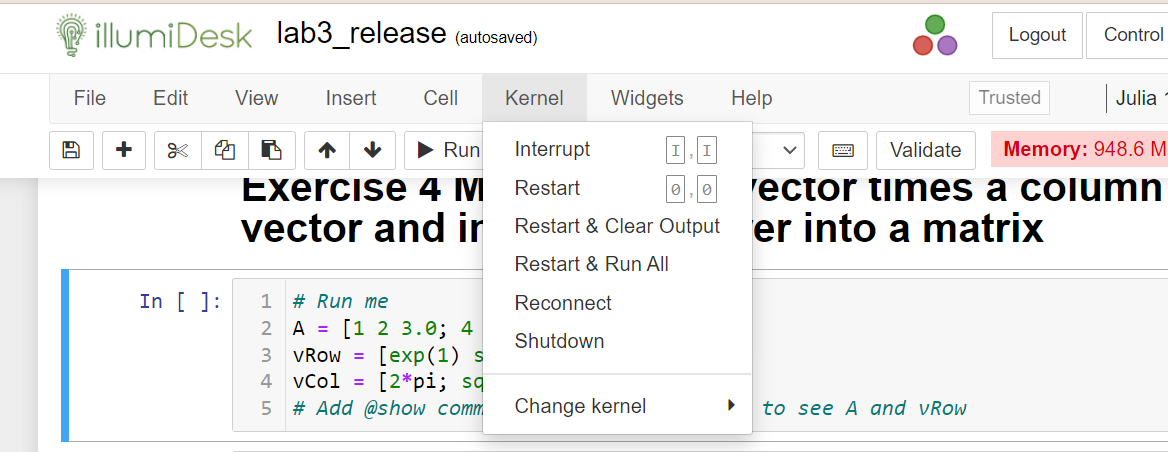
\includegraphics[width=0.9\columnwidth]{Chap00/KernelDropDownMenu.png}}%
}


\begin{itemize}
    \item Click on the Kernel tab, to get the above dropdown menu. Click on the \texttt{Restart \& Clear Output} \textbf{or} \texttt{Restart \& Run All}.
    \item Neither of these erases any code in your Input Cells. Your work is safe! 
    \item \texttt{Restart \& Clear Output} Stops and restarts the program that is running your notebook and clears all of the output cells. You then need to start from the top cell in your notebook (or other relevant location) and re-run each cell to redefine your variables because \textbf{the value of each variable has been ``erased''}. Once again, all of your code is still there. 
    \item \texttt{Restart \& Run All} does all of the above and re-runs every cell in your notebook automagically (not a typo). You'll have to experiment with these two options to see which one you like best. 
\end{itemize}

\textcolor{red}{\bf Sometimes the above is not enough and you need a ``nuclear option''.} Step 1 is to return to Canvas and select IllumiDesk. You can see that I am currently working in the F-21 Canvas site.\\

\setlength{\fboxrule}{3pt}%
	\centerline{ \fbox{ 
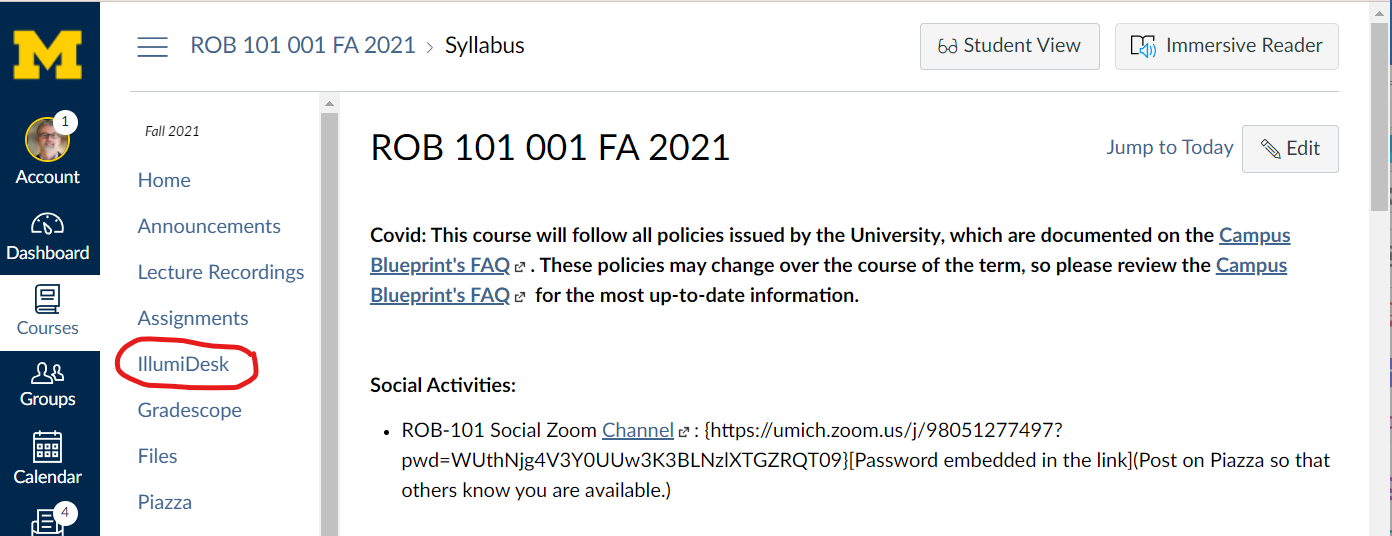
\includegraphics[width=0.9\columnwidth]{graphics/Chap00/IllumiDesk.png}}%
}
\vspace*{.2cm}

Step 2 is to hit the \textbf{Stop My Server} button. Be patient. It takes some time to close all of the related processes. When the red button goes away, then hit the \textbf{Start My Server} button, watch your server ``spool up'', re-open your file and proceed. If you return to your previously opened file, it may work, but it may not. I find it best to open a fresh copy of the file. \textcolor{red}{\bf Personally, I do not close my previously opened file until I am sure that I do not need to copy any lines of code from it.} You'll arrive at your own file management etiquette!\\

\setlength{\fboxrule}{3pt}%
	\centerline{ \fbox{ 

\includegraphics[width=0.9\columnwidth]{graphics/Chap00/StopMyServer.png}}%
}



\section{(Optional Read) Why was Julia Created?}


The following material is from \url{https://juliadatascience.io/julia_accomplish}: 
``We are greedy: we want more. We want a language that’s open source, with a liberal license. We want the speed of C with the dynamism of Ruby. We want a language that’s homoiconic, with true macros like Lisp, but with obvious, familiar mathematical notation like Matlab. We want something as usable for general programming as Python, as easy for statistics as R, as natural for string processing as Perl, as powerful for linear algebra as Matlab, as good at gluing programs together as the shell. Something that is dirt simple to learn, yet keeps the most serious hackers happy. We want it interactive and we want it compiled.''
% \begin{lstlisting}[language=Julia,style=mystyle]

% \end{lstlisting}
% \textbf{Output} 
% \begin{verbatim}

% \end{verbatim}
